\label{systemDesign}
The system used in this project was designed to take advantage of the hardware-software interfaces of the Zynq SoC. An overall block diagram of the system is shown in Figure \ref{systemBD} below. The design was broken down into several functional blocks. These include the sensor hardware shown in red, programmable logic (PL) shown in green, and programmable software (PS) shown in blue. 

\begin{figure}[H] 
	\centerline{
	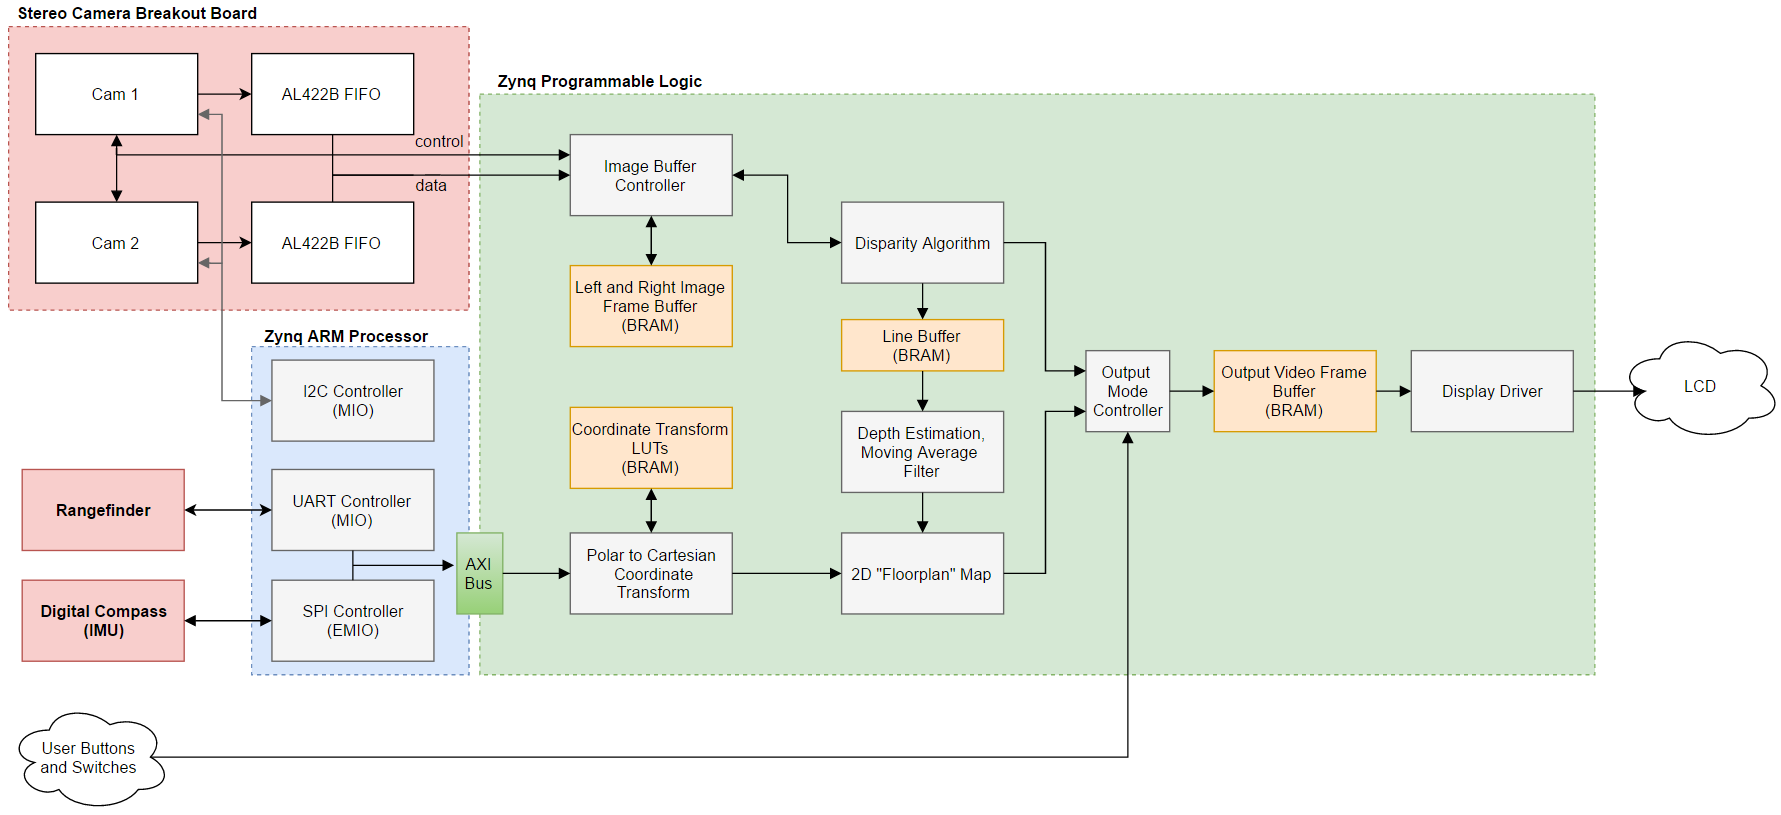
\includegraphics[width=1.25\linewidth]{full_blockdiag.png}
	}
	\caption{System Block Diagram}
	\label{systemBD}
\end{figure}

The majority of the design was implemented in PL rather than in PS in order to maximize the amount of calculations performed in parallel. For ease of integration, communication with the rangefinder and digital compass was handled using the ARM processor of the Zynq SoC, as  pre-configured SPI and UART peripheral drivers were available through Xilinx. Data obtained through these interfaces was then pre-processed before being passed to the FPGA fabric, allowing for rangefinder distance data to be rotated based on the digital compass heading. A customized Advanced eXtensible Interface (AXI) peripheral bus was then used to pass said data from the ARM processor to the programmable logic. Within the programmable logic, a pair of lookup tables were used to convert pre-rotated rangefinder distance data from Polar to Cartesian coordinates to create a 2D "floorplan" of the sensor suite's environment.
\par
Along with pre-processing compass and rangefinder data, the PS was used to initialize each camera module for manual trigger mode per an I$^2$C peripheral driver at startup. Following this initialization sequence the PS continuously gathered new data samples from the rangefinder and compass. Simultaneously, a separate PL module triggered new image captures from the stereo camera pair. Since the camera modules immediately output their image data after a new trigger sequence, a customized stereo camera printed circuit board was designed with attached image buffer integrated circuits (ICs) for temporarily storing image data. This intermediate buffering stage allowed the programmable logic to read image data into local memory using separate clock domains, easing the overall timing requirements of the image processing pipeline. After stereo camera image data had been read into on-chip memory, a disparity module was then used to calculate the relative offset between objects contained in the stereo image pair. The resultant disparity image was stored in a video frame buffer for VGA display. A portion of this data was also stored in a separate memory buffer for correlation with data from the 2D scanning laser rangefinder. 
\par
In order to correlate disparity data with 2D depth information from the scanning laser rangefinder, several horizontal lines of pixel data from the disparity algorithm were passed through a moving average filter. This filter was used to smooth the disparity depth data, as well as to account for differences in the field of view of each sensor. After this processing stage, the 2D disparity and laser rangefinder data was combined directly. Depending on the status of the ZedBoard's user switches, this 2D floorplan map was then passed to the output video buffer for external display.
\par
The system implementation is explored further in the next chapter.